\section{光的粒子性}

\begin{quotation}
``我们之所以知道光是由粒子组成,是因为我们使用一种非常灵敏的仪器,当光照射这个仪器时,仪器就``嗒''``嗒''``嗒''作响。
如果光变暗了,响声还是那么强,只是响的次数变少了。''\qquad 费曼
\end{quotation}

\subsection{历史回顾}

关于光本性的争论, 持续了很长时间, 牛顿(Newton)认为是粒子,
并解释了光的直线传播, 光的折射现象,
但粒子说无法解释光的干涉和衍射现象\footnote{我们这么说,
牛顿本人未必会同意, 在他看来牛顿环恰恰是``光是粒子''的证据,
但牛顿没法给出计算条纹间距的公式,
而``波动说''可以给出。}。惠更斯(Huygens)认为是机械波, 可以解释:
直线传播、折射、干涉、衍射现象。``光的波动说''因为能解释干涉、衍射现象而稍占上风。

1850年, 麦克斯韦(Maxwell)在法拉第(Faraday)电磁学实验研究基础上,
提出了麦克斯韦方程组, 由麦克斯韦方程组可以推出电磁场波动方程,
电磁波传播速度恰好为光速$c$, 这样, 光学和电磁学就被统一起来,
光波就是电磁波。

\index{Electromagnetic wave: 电磁波}

\begin{eqnarray*}
\nabla  \cdot D = 0,\nabla  \times E =  - \frac{{\partial B}}{{\partial t}},\nabla  \cdot B = 0,\nabla  \times H & = & \frac{{\partial D}}{{\partial t}}  \\
\left( {\nabla ^2  - \frac{1}{{c^2 }}\frac{{\partial ^2 }}{{\partial t^2 }}} \right)\left\{ {\begin{array}{*{20}c}
   {\mathord{\buildrel{\lower3pt\hbox{$\scriptscriptstyle\rightharpoonup$}}
\over E} }  \\
   {\mathord{\buildrel{\lower3pt\hbox{$\scriptscriptstyle\rightharpoonup$}}
\over B} }  \\
\end{array}} \right\} & =  & 0
\end{eqnarray*}

通常我们所说的光就是特定频率的电磁波,
我们可简要地回顾一下电磁波谱的概念\footnote{参考, 杨福家,
《原子物理学》, pp248.}:

\begin{figure}[h]
\begin{center}
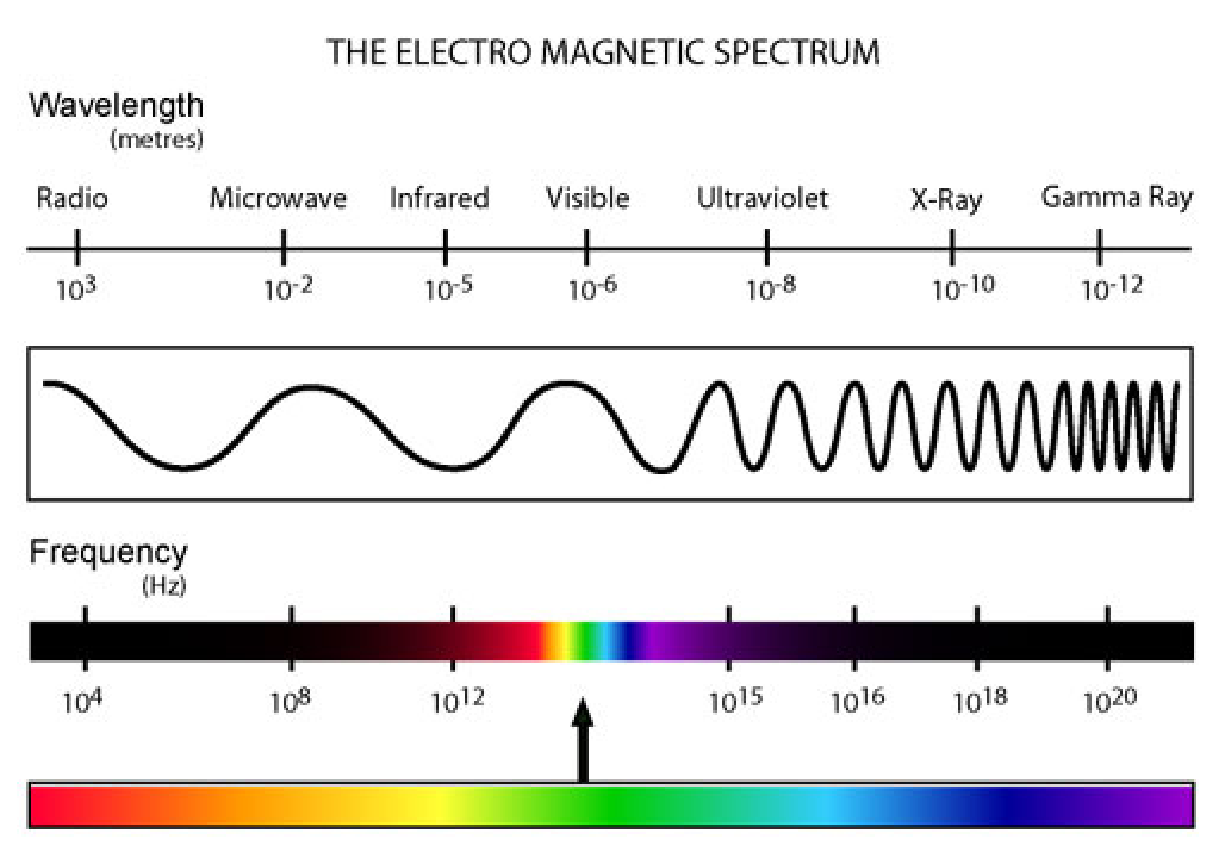
\includegraphics[width=10cm]{Duality/em-spectrum.ps}
\caption{电磁波谱}
\end{center}
\end{figure}

\index{Electromagnetic spectrum: 电磁波谱}

\begin{itemize}
  \item gamma-射线:波长最短(0.01埃左右),能量最高;
  \item X-射线:波长(0.1-10埃),恰好和晶格尺寸吻合,广泛地用于物质结构测定,无损检测,医疗诊断等;能量:$k$eV-$10^5$eV
  \item 紫外(ultraviolet):波长(纳米-百纳米)
  \item 可见光(visible light):波长(几百纳米量级)
  \item 红外(infrared):波长(微米-毫米)
  \item 微波(microwave):波长(毫米,厘米,分米)
  \item 电磁波:波长大于0.1米
\end{itemize}


19世纪末, 为了把Maxwell的电磁理论与Newton的经典力学统一起来,
科学家提出以太学说, 设想光波/电磁波象机械波一样借助某种介质,
即``以太''传播。 以太学说的困难直接导致Einstein提出狭义相对论,
这是量子力学外, 近代物理学又一重大发现。

狭义相对论主要结论:

\index{Special relativity: 狭义相对论}

\begin{enumerate}
    \item 相对论质量:$m = \frac{{m_0 }}{{\sqrt {1 - {\textstyle{{v^2 } \over {c^2 }}}} }}$, $m_0$静止质量。
    \item 动量能量关系:$E = mc^2  = \frac{{m_0 c^2 }}{{\sqrt {1 - {\textstyle{{v^2 } \over {c^2 }}}} }},E^2  = p^2 c^2  + m_0 ^2 c^4 $
    \item 动能:$K = E - m_0 c^2$
\end{enumerate}

\subsection{光电效应}

\index{Hertz's experiment: 赫兹实验}

1887年,赫兹(Hertz)实验证明光波就是电磁波:赫兹用莱顿瓶进行放电实验,
发现了电磁波,电磁波有$\textbf{E}$和$\textbf{B}$的分量,
有散射、干涉、反射等波动特征,传播速度等于光速。赫兹实验验证了Maxwell的理论,并最终判定Newton的光粒子说失败。
但具有讽刺意义的是,在这个``决定性''的实验中,赫兹发现当紫外光(单频)照在负极上时,放电就比较容易发生,
这正是发生光电效应的原因。后来爱因斯坦对光电效应的解释说明:要正确解释光电效应,就必须承认光是粒子。

\begin{figure}[h]
\begin{center}
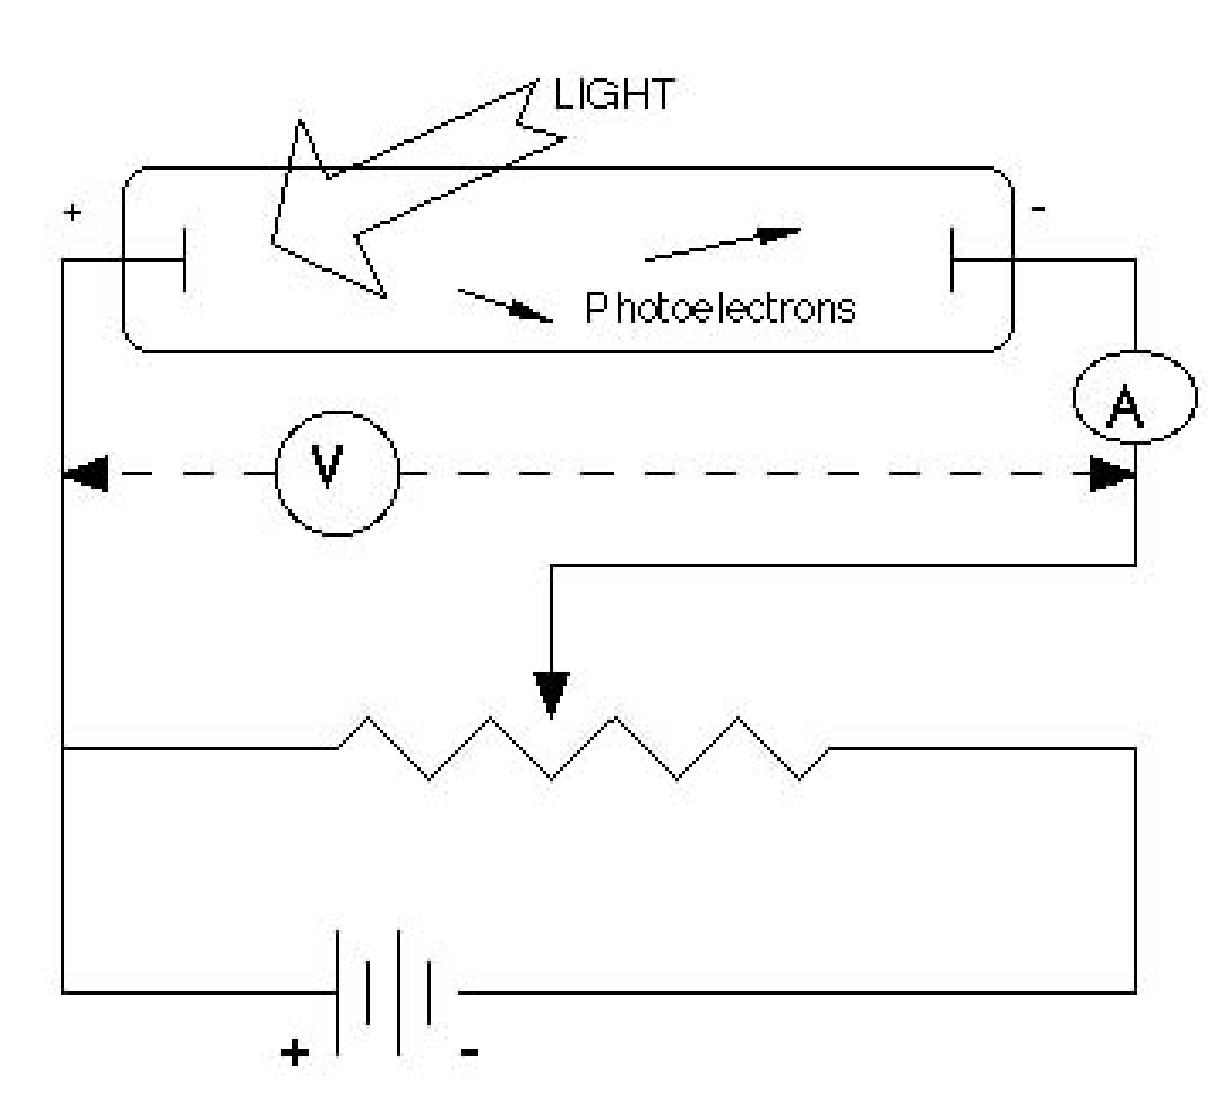
\includegraphics[width=8cm]{Duality/3-1.ps}
\caption{光电效应示意}
\end{center}
\end{figure}

光电效应的实验规律:

\index{Photoelectric effect: 光电效应}

\begin{enumerate}
    \item 饱和电流$I$:随着电压的变大,光电流趋于饱和值(I与单位时间内阴极放出的光电子数成正比)。
饱和电流与光强成正比,或说单位时间内由阴极放出的光电子数与光强成正比。
    \item 存在遏止电压(stopping voltage)$V_0$,遏止电压与光强无关。说明光电子存在最大动能:${\textstyle{1 \over 2}}mv_0 ^2  = eV_0 $。
    \item 存在截止频率(threshold frequency)$\nu _0$,入射光束为单频,改变其频率,发现对应遏止电压随之变化,当入射光低于某频率$\nu _0$时,$V_0$ 减为0,无论光强多大,光电效应不再发生。说明截止频率$\nu _0$与阴极的物性有关。
    \item 弛豫时间$\tau$:弛豫时间与光强无关,光电子几乎在光照瞬间产生,$\tau  < 10^{ - 9} s$。
\end{enumerate}

光的波动理论无法解释光电效应:

(1)按照光的电磁波理论,光强正比于电磁场振幅的平方,电子在变化的电磁场中作受迫振动,
电子振幅足够大时则脱离金属而逸出,类似我们荡秋千时在伙伴的推动下越荡越高的过程。所以光强越大,照射时间越长,
则光电子越容易逸出。但实验表明,光电子是否逸出只与入射光频率有关,而对应弛豫时间很短,无论光强多弱,
整个过程几乎在瞬间完成。

(2)更深入地讨论,如入射光频率与电子振动本征频率接近则发生共振现象,光电子应很快逸出,
但一旦大于此本征频率,电子受迫振动振幅应减小,从而较难逃逸出去,但实验表明一旦入射光超过截止频率,都会有光电效应发生。

\index{photon: 光子}

1905年,受普朗克量子假说启发,爱因斯坦提出光量子假说,正确解释了光电效应:光的能量不象波动理论所想象那样,
是连续分布的(正比于电磁场振幅平方,并分布在空间中),而是集中在一些叫光子(photon)的粒子上,
光子的能量服从普朗克关系:$\varepsilon  = h\nu $。

根据能量守恒, 得到爱因斯坦公式:

\begin{equation}\label{Einstein phtoemission}
   h\nu  = \frac{1}{2}mv_0 ^2  + A = eV_0  + A
\end{equation}

其中:$A = h\nu _0 $,是逸出功(work function),与材料的性质有关。

爱因斯坦对光电效应的解释是:

(1)电磁波能量被集中在光子身上,而不是象波那样散布在空间中,
所以电子可以集中地、一次性地吸收光子能量,所以对应弛豫时间应很短,是瞬间完成的。

(2)所有同频率光子具有相同能量,光强则对应于光子的数目,光强越大,光子数目越多,所以遏止电压与光强无关,
饱和电流与光强成正比。

(3)光子能量与其频率成正比,频率越高,对应光子能量越大,所以光电效应也容易发生,光子能量小于逸出功时,则无法激发光电子。


\subsection{X射线}

光电效应中, 电磁波可以将能量转移给电子并将电子激发出来,
与之相反的过程则是电子撞击物质, 并发出电磁辐射, 即X射线。
X射线辐射:$eV_0  \to h\nu  + e$,可看作是光电效应:$h\nu  + e \to eV_0 $的逆过程。

\index{X-ray: X射线}

1895年,伦琴(Roentgen)发现X射线\footnote{参考杨福家《原子物理学》第246页;}。伦琴是历史上第一个诺贝尔物理奖得主。在19世纪末本来物理学家们认为已经没有什么现象是经典理论无法解释的了,伦琴的发现着实使当时的人们大吃一惊,一种神秘的射线竟然可以穿透人体,并使人身体内部的构造成像。这提示当时的物理学家,求知的过程是没有穷尽的,物理学还远未终结。

在电磁波谱中,X射线在紫外与Gamma射线之间,波长范围一般在0.001nm但1nm,比0.1nm短的称为硬X射线,比0.1nm长的,称软X射线。\footnote{关于电磁波谱:
参考杨福家《原子物理学》第248页;}

\begin{figure}[h]
\begin{center}
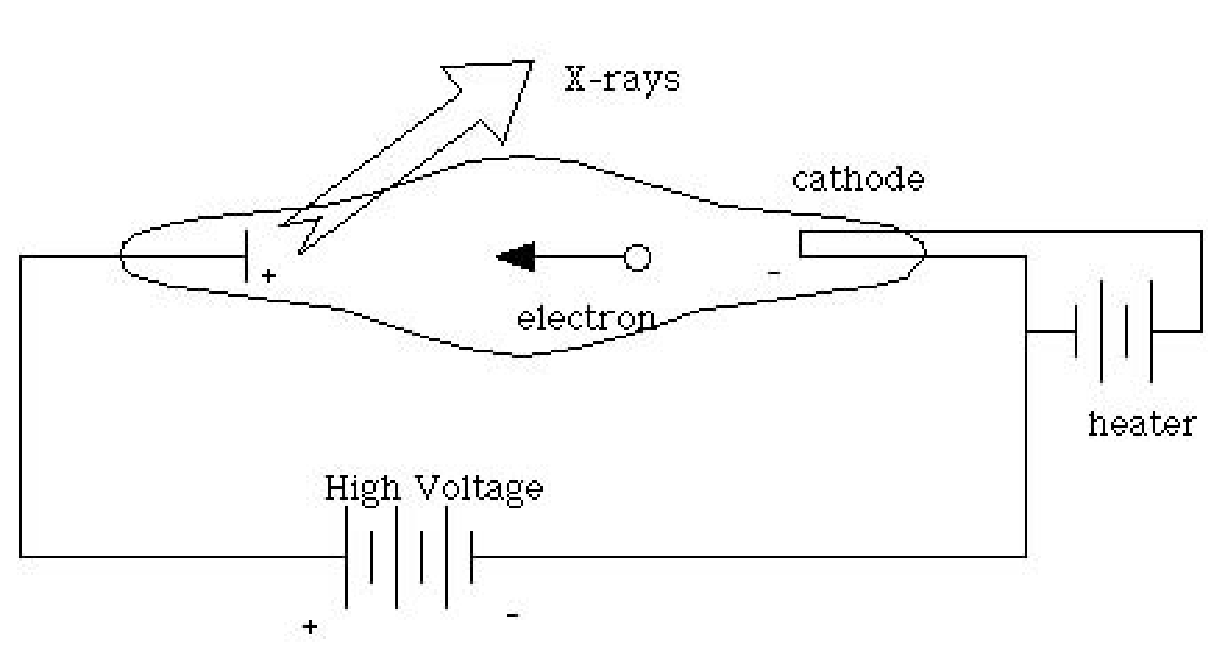
\includegraphics[width=9cm]{Duality/3-2.ps}
\caption{X射线示意}
\end{center}
\end{figure}

根据经典电动力学知识,高速运动电子撞击金属靶,急剧减速,这个过程中必将发生电磁辐射,称为轫致辐射,或刹车辐射。
(轫致辐射的详细理论需要量子电动力学QED的知识)
考虑入射电子与耙原子核之间库仑相互作用,轫致辐射强度反比于入射带电粒子质量平方,正比于靶核电荷的平方
($I \propto \frac{{Z^2 }}{{m_e ^2 }}$),由于带电粒子速度是连续变化的,因此X射线辐射有连续谱的性质。

实验观测到连续谱的形状与靶的材料无关,但存在一个最小波长$\lambda _{\min}$(或最大频率$\nu _{\max }  = \frac{c}{{\lambda _{\min } }}$),其数值仅依赖于加速电压$V_0$,而与耙材料无关。根据普朗克光量子假说:$\varepsilon  = h\nu $,$h\nu _{\max }  = eV_0 $,即最大频率对应于电子动能完全转成辐射能(光子能量)的情况,

\begin{equation}
\lambda _{\min }  = \frac{{ch}}{{eV_0 }}
\end{equation}

这个$\lambda _{\min }$称为量子极限。

\begin{figure}[h]
\begin{center}
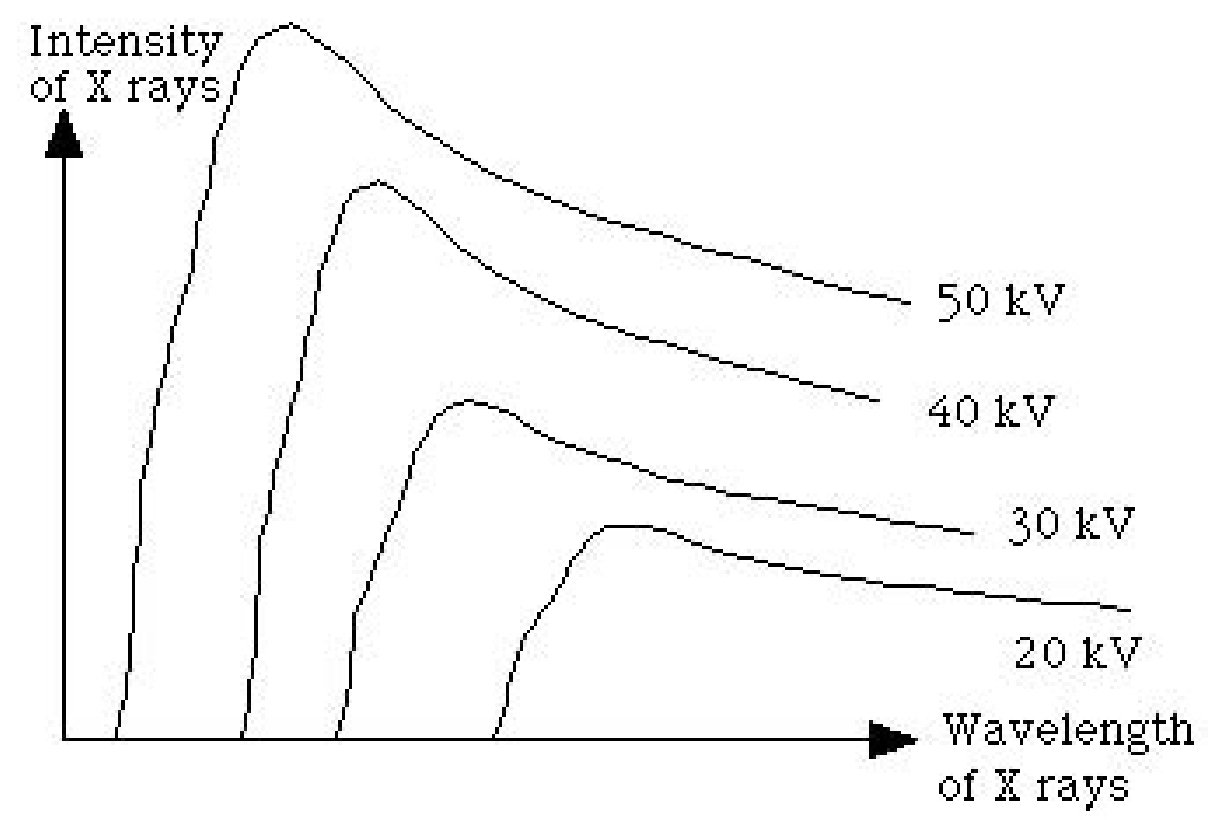
\includegraphics[width=6cm]{Duality/3-3.ps}
\caption{X射线的量子极限}
\end{center}
\end{figure}

实验观察发现,在连续谱上面还存在一些``尖峰'',是特征辐射产生的X射线谱,其对应位置与外加电压无关,
各不同元素的特征X射线谱有类似的结构,但波长位置各不相同,正如指纹可作为人的特征,特征X射线是元素的``指纹''。
特征辐射是经典电动力学所无法解释的,它与原子的内部结构有关系,我们在以后的课程中再给出解释。


\begin{figure}[h]
\begin{center}
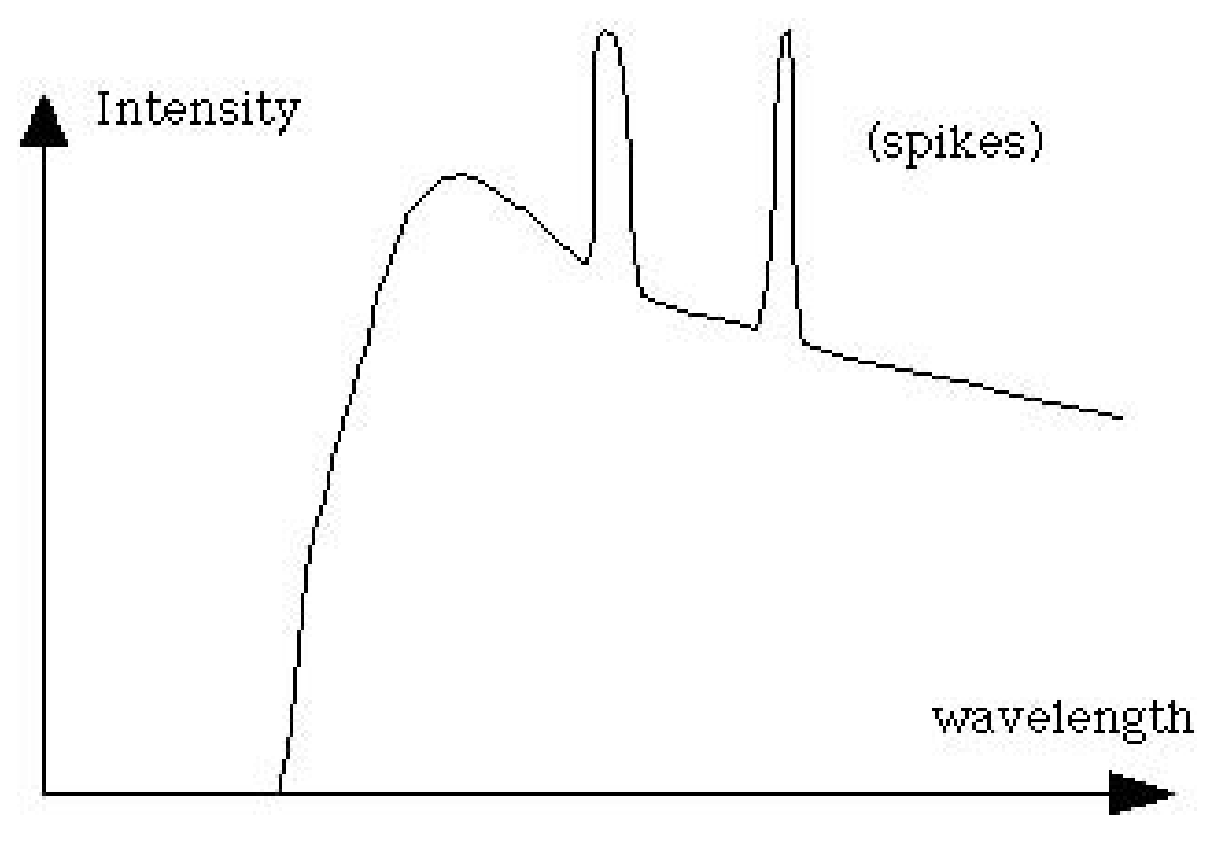
\includegraphics[width=6cm]{Duality/3-4.ps}
\caption{X射线谱的特征辐射}\label{xray-spec}
\end{center}
\end{figure}

特征辐射按辐射的硬度(穿透能力)递减顺序可将特征辐射标记为K、L等系列,并可再细分为$K_\alpha  ,K_\beta  ...,L_\alpha  ,L_\beta  ,...$等谱线\footnote{参考杨福家《原子物理学》第259页;}。

\subsection{X射线衍射}

\index{X-ray diffraction: X射线衍射}

X射线经过大小与其波长类似的狭缝时,将发生衍射现象。对于X射线而言,其波长的数量级为$0.1nm$,很难人工制备这么小尺寸的光栅。
劳厄首先建议用晶体这个天然的光栅用来观察X射线的衍射。

\begin{figure}[htbp]
\begin{center}
\includegraphics[width=9cm]{Duality/BraggPlaneDiffraction.png}
\caption{布拉格公式}
\label{BraggPlaneDiffraction}
\end{center}
\end{figure}

X射线衍射满足布拉格公式\index{Bragg's formula: 布拉格公式}:

\begin{equation}\label{3-1}
2d \sin \theta = n\lambda, n = 1, 2, ...
\end{equation}

$d$是晶格间的间距,相邻两束光的光程差是$2d \sin \theta$。在布拉格公式中,如图\ref{BraggPlaneDiffraction}, $d$,
$\theta$和$\lambda$都是确定的, 很难有满足此条件的$n$存在,
即很难观察到衍射峰。为克服这个困难,
我们一般用连续的X射线谱(改变$\lambda$)对晶体结构进行分析,
称为\textbf{劳厄法}。
或者我们还可通过转动晶体(改变$\theta$)对晶体结构进行分析,
称为\textbf{旋转晶体法}。 但旋转晶体会涉及到复杂的机械装置,也不方便。

\begin{figure}[htbp]
\begin{center}
\includegraphics[width=9cm]{Duality/DebyeScherrer.png}
\caption{粉末法示意}
%\label{default}
\end{center}
\end{figure}

如果单色X射线被晶体粉末(或多晶)散射,
由于晶面取向是杂乱无章的,
那些恰好满足布拉格条件的晶面取向(对应特定散射角$\theta$),
将发生相长干涉, 形成衍射条纹, 这种方法称为\textbf{德拜-谢乐法}(或粉末法)。

X射线衍射是重要的结构测量手段,
X射线衍射技术最了不起的发现是导致了DNA双螺旋结构的发现,
从此关于生命现象的研究也建立在原子和分子的水平上了。图\ref{franklin1951}是罗莎琳·富兰克林(Rosalind
Franklin)在1951年得到的,
这是对克里克(Crick)和沃森(Watson)提出的DNA双螺旋结构的直接证据,
图中央由黑点组成的``X形图样''是由于双螺旋结构造成的;
上下两端``弧形图样''是由于碱基每隔$3.4$埃上升一周期造成的。

\begin{figure}[h]
\begin{center}
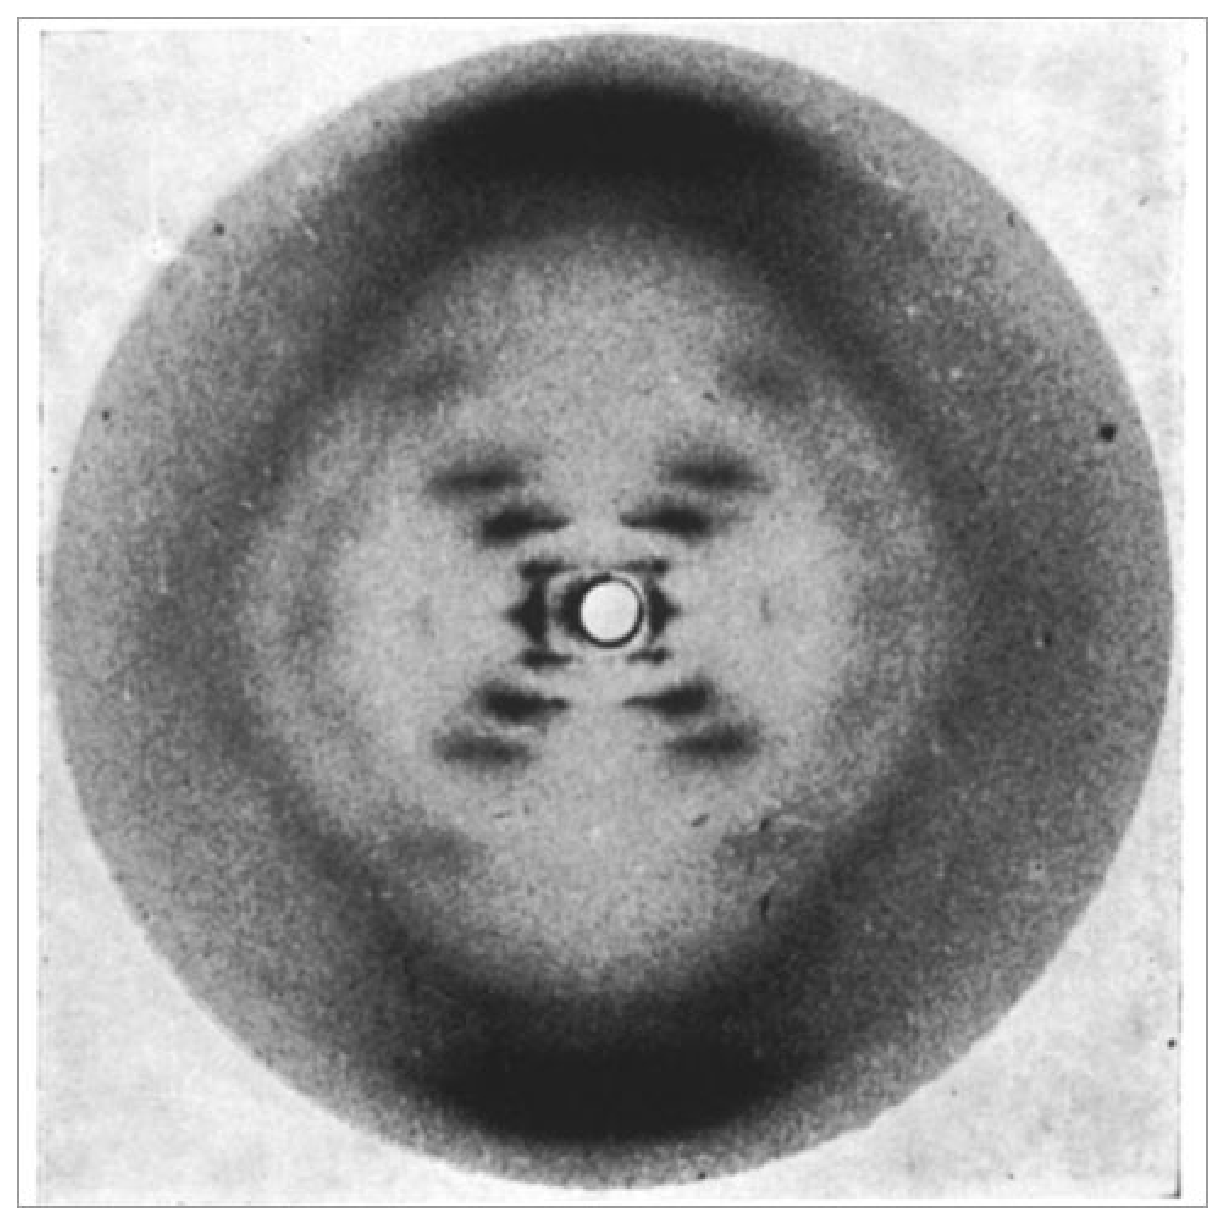
\includegraphics[width=5cm]{Duality/pbs-photo51.ps}
\caption{DNA双螺旋结构的X射线衍射图像}\label{franklin1951}
\end{center}
\end{figure}

\index{DNA Double Helix: DNA双螺旋}

实际上克里克和沃森在构造他们的双螺旋结构的过程中事先就知道了富兰克林和威尔金斯(Wilkins)的X射线衍射数据,
并因此而受益\footnote{``In constructing their model, Watson and
Crick were helped by advance knowledge of X-ray data obtained by
Rosalind Franklin and Maurice Wilkins at King's College London.
These results - and additional data and reasoning supporting the
Cambridge structure - were published in the same issue of Nature.''

参考: ``The Cavendish Laboratory and structural biology'',
\url{http://physicsworld.com/cws/article/print/17020}}。
克里克和沃森的文章,
富兰克林的文章和威尔金斯的文章都发表在自然杂志的同一期(\emph{Nature}
\textbf{171}, 1953)上,
但威尔金斯得到的X射线衍射图像明显没有富兰克林得到的图像清晰。
当克里克, 沃森和威尔金斯在1962年获得诺贝尔生理和医学奖的时候,
富兰克林已经英年早逝了, 她死于1958年, 只有37岁。

目前大多数实验室采用同步辐射加速器作为X射线源。在磁场的作用下高速运动的电子在同步辐射加速器或储存环(Storage ring)里转圈,在电子运动的切线方向会辐射出高质量的同步辐射(synchrotron radiation)。

\begin{figure}[htbp]
\begin{center}
\includegraphics[width=9cm]{Duality/synchrotron.png}
\caption{同步辐射}
%\label{default}
\end{center}
\end{figure}


同步辐射的优点是\footnote{参考杨福家《原子物理学》第266页。关于同步辐射技术, 更多请阅读: 

维基百科词条 Synchrotron radiation:\url{http://en.wikipedia.org/wiki/Synchrotron_radiation}

徐克尊, 《高等原子分子物理学》,科学出版社, 第5.5节。}:

\begin{enumerate}
    \item 功率大;
    \item 能谱宽;
    \item 方向性好。
\end{enumerate}

\begin{figure}[h]
\begin{center}
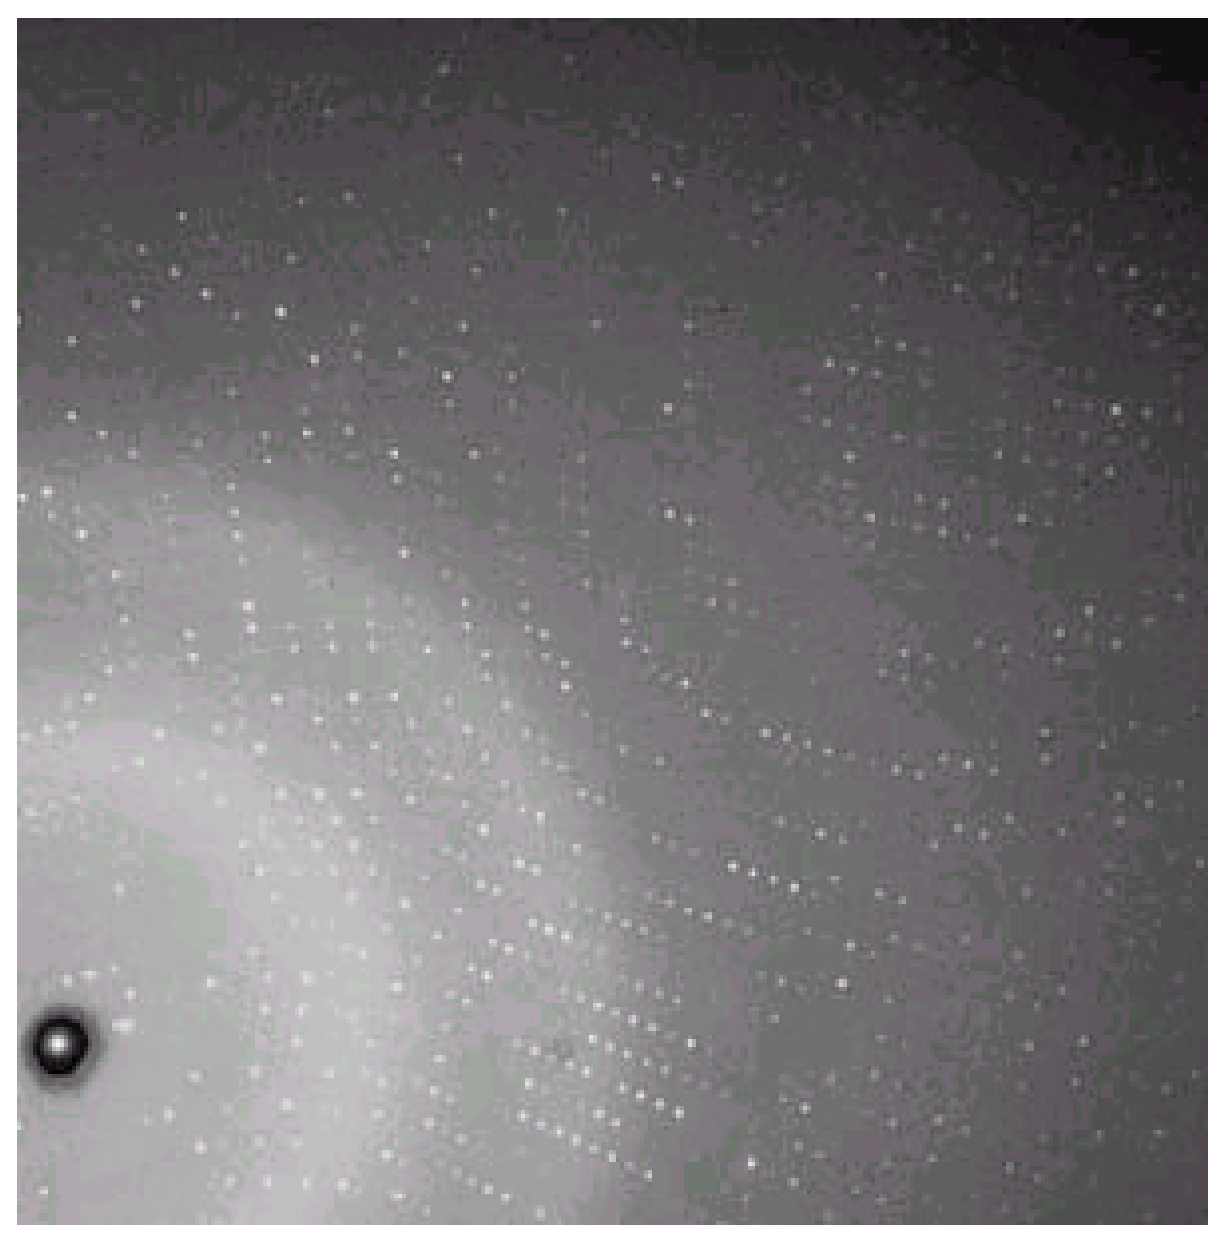
\includegraphics[width=5cm]{Duality/xray.ps}
\caption{蛋白质晶体X射线衍射图像}
\end{center}
\end{figure}


\subsection{康普顿散射}

如果光子是粒子,除具有在空间集中分布的能量外,还应具有在空间集中分布的动量。

爱因斯坦提出光子具有动量\footnote{根据爱因斯坦质能关系: $\varepsilon
= h\nu  = mc^2 ,p = mc = \frac{\varepsilon }{c} = \frac{{h\nu }}{c}
= \frac{h}{\lambda }$}:

\begin{equation}\label{Einstein momentum of photon}
    p = \frac{h}{\lambda }
\end{equation}


\index{Compton scattering: 康普顿散射}

康普顿(Compton)在研究X射线与物质散射的实验中,
发现X射线被轻原子量的物质散射后, 波长有变长的现象。
康普顿散射实验中用的靶的材料是石墨, 由于石墨正好位于周期表的中间,
因此石墨的外层电子束缚的不太结实,
使电子在被高能光子(X射线能量较高)散射前恰好可看作是静止的,
同时又是自由的\footnote{如果使用金属做靶的话,
外层电子是自由的、属于整个金属共有并遵从费米分布。
此时我们可通过康普顿散射轮廓(Compton
Profile)来推测金属内自由电子的动量分布,
并验证其确实满足费米分布。更多, 请阅读: 杨福家, 《原子物理学》,
第三版, pp275-276.}。
假设光子具有动量,碰撞过程中应满足能量与动量守恒,光子与静止电子
之间会发生动量和能量转移, 使光子频率变小,波长变长。

\begin{figure}[h]
\begin{center}
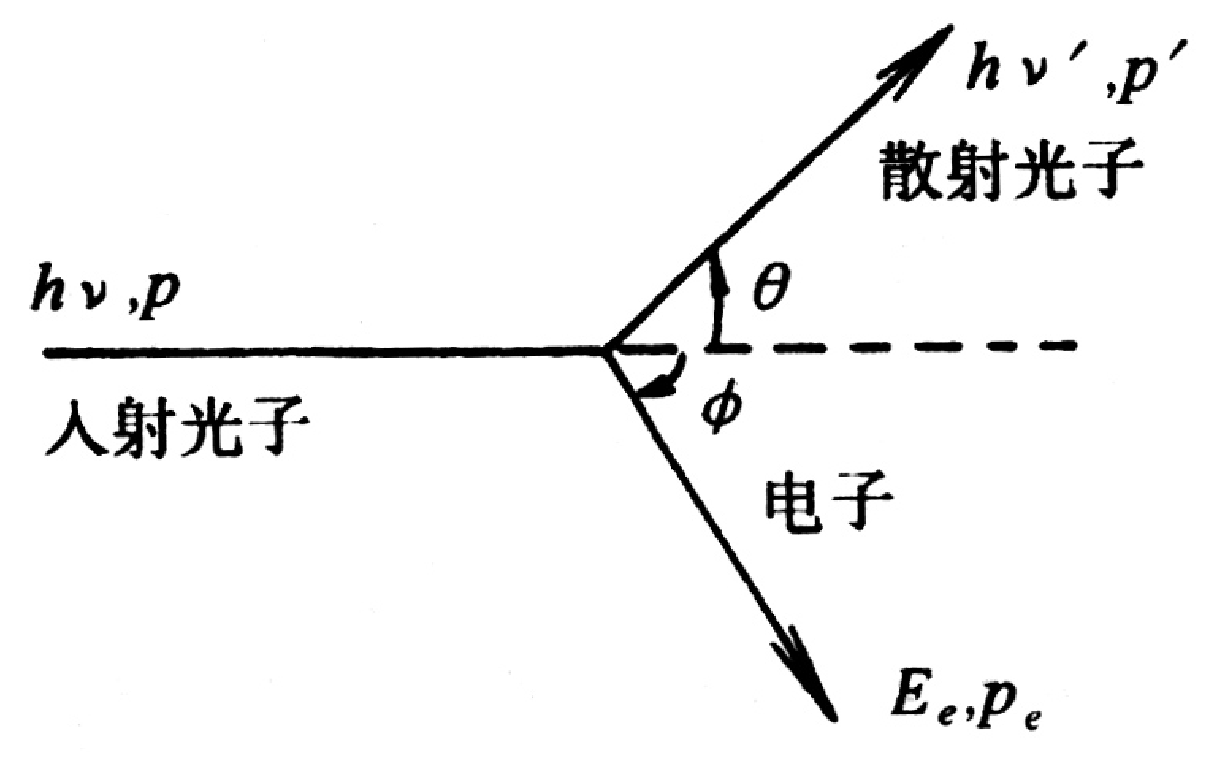
\includegraphics[width=6cm]{Duality/3-5.ps}
\caption{康普顿散射示意}
\end{center}
\end{figure}

碰撞前电子速度很小,视为静止,由于入射光子能量很高(远大于电子在原子中束缚能),所以电子可视为自由电子。


入射光子:$h\nu ,p$;散射光子:$h\nu ',p'$;碰撞后电子:$E_e ,p_e $;$p,p'$夹角$\theta$;$p,p_e $
夹角$\phi$
由于碰撞过程中动量守恒$p = p' + p_e $,碰撞只能发生在同一平面中。

\begin{equation}
\left\{ \begin{array}{l}
 h\nu  + m_e c^2  = h\nu ' + E_e  \\
 p = p' + p_e  \\
 \end{array} \right.
\end{equation}

即:

\begin{equation}
\left\{ \begin{array}{l}
 E_e  = h(\nu  - \nu ') + m_e c^2  \\
 p_e  = p - p' \\
 \end{array} \right.
 \end{equation}

\index{Special relativity: 狭义相对论}

利用相对论能量动量关系:

\begin{equation}
E_e ^2  = p_e ^2 c^2  + m_e ^2 c^4 
\end{equation}

将上式代入化简为:

\begin{equation}
\left[ {h(\nu  - \nu ') + m_e c^2 } \right]^2  = (p - p')^2 c^2  + m_e ^2 c^4 
\label{ComptonScatteringDerivation}
\end{equation}

其中:

\begin{eqnarray*}
(p - p')^2 &=&  \left| p \right|^2  + \left| {p'} \right|^2  -
2\left| p \right| \cdot \left| {p'} \right| \cdot \cos \theta \\
 {} & = & \left( {\frac{{h\nu }}{c}} \right)^2  + \left( {\frac{{h\nu '}}{c}}
\right)^2  - 2\left( {\frac{{h^2 \nu \nu '}}{{c^2 }}} \right)\cos
\theta \\
{} & = & \frac{{h^2 }}{{c^2 }}\left( {\nu ^2  + \nu '^2  - 2\nu \nu
'\cos \theta } \right)
\end{eqnarray*}

公式(\ref{ComptonScatteringDerivation})的左侧(LHS):

\begin{equation*}
\left[ {h(\nu  - \nu ') + m_e c^2 } \right]^2  = h^2 (\nu ^2  + \nu '^2  - 2\nu \nu ') + m_e ^2 c^4  + 2m_e hc^2 (\nu  - \nu ')
\end{equation*}

公式(\ref{ComptonScatteringDerivation})的右侧(RHS):

\begin{equation*}
(p - p')^2 c^2  + m_e ^2 c^4  = h^2 (\nu ^2  + \nu '^2  - 2\nu \nu '\cos \theta ) + m_e ^2 c^4 
\end{equation*}

由“LHS = RHS”化简可得:

\begin{equation*}
 - 2h^2 \nu \nu ' + 2m_e hc^2 (\nu  - \nu ') =  - 2h^2 \nu \nu '\cos \theta
\end{equation*}

即:

\begin{equation*}
m_e c^2 (\nu  - \nu ') = h\nu \nu '(1 - \cos \theta )
\end{equation*}

进一步化简:

\begin{equation*}
h(1 - \cos \theta ) = m{}_ec^2 \left( {\frac{1}{{\nu '}} - \frac{1}{\nu }} \right)
\end{equation*}

最后得到:

\begin{equation*}
\frac{1}{{\nu '}} - \frac{1}{\nu } = \frac{h}{{m_e c^2 }}(1 - \cos \theta )
\end{equation*}

由于$\lambda  = \frac{c}{\nu }$,两边同时乘$c$,得到康普顿散射公式:

\begin{equation}\label{Compton's formula}
    \Delta \lambda  = \lambda ' - \lambda  = \frac{h}{{m_e c}}(1 - \cos \theta )
\end{equation}


\index{Compton wavelength: 康普顿波长}

可定义电子的康普顿波长:

\begin{equation}
\lambda _c  = \frac{h}{{m_e c}} = 2.43 \times 10^{ - 3} nm
\end{equation}

\subsubsection{实验结果}


\begin{figure}[h]
\begin{center}
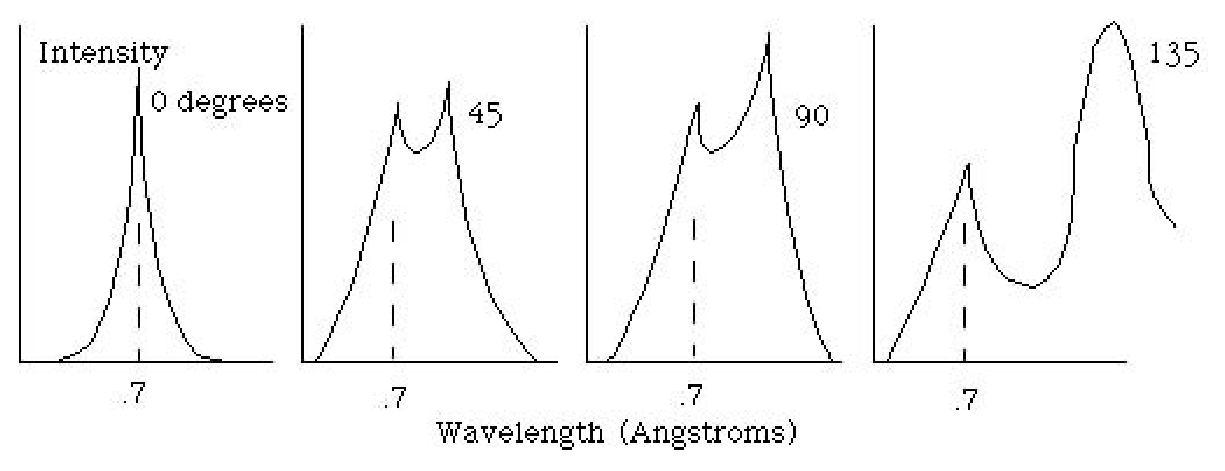
\includegraphics[width=10cm]{Duality/3-6.ps}
\caption{不同角度时的康普顿散射}
\end{center}
\end{figure}

\begin{enumerate}
    \item 根据康普顿散射公式,$\Delta \lambda  = \lambda ' - \lambda  \ge 0$,即散射后波长变长了。
    \item 质子的康普顿波长比电子的小约2000倍,这是为什么我们只考虑了X射线与电子的散射,而没考虑与原子核的散射。
    \item $\Delta \lambda $与入射波波长无关,只决定于散射角$\theta$,$\theta  = 180^o $时最大。\footnote{当$\theta  = 180^o $时,$\Delta \lambda  = 2\frac{h}{{m_e c}} = 0.0049nm$}
    \item 计算中假设电子是自由的,实际上大多数内层电子被束缚很紧,光子同这样的电子碰撞,相当于和整个原子碰撞,
所以动量能量转移很小,所以在散射谱中总存在$\lambda$这条谱线。
\end{enumerate}


\textbf{小结}:黑体辐射、光电效应和康普顿散射表明光具有粒子的特性:
$\varepsilon = h\nu ,p = h/\lambda
$;但光的波动理论早已被干涉、衍射等现象证实,
这样光就具有粒子和波动的双重属性, 这种性质称为:
\textbf{波粒二象性}(Wave-particle duality)。

\index{Wave-particle duality: 波粒二象性}

\subsection*{练习}

\begin{enumerate}
%  \item 普朗克常数($h$)一般用$J \cdot s$为单位表示,现在请换为用$MeV \cdot s$表示。
  \item 频率为$8.5 \times 10^{15} Hz$的光照射在金属表面上,如发射出光电子的动能为$1.7eV$, 求金属的逸出功是多少?(把结果用电子伏$eV$表示)
  \item 要分辨$0.1nm$ 尺度的物质结构,我们需要使用多强的X-射线(用电子伏表示)?
  \item 假设$60W$的灯泡主要发射波长$\lambda = 1000 nm$的光,求每秒发射出的光子数;人的眼睛可分辨,比如最少五个光子的亮光,假设眼睛的瞳孔直径是$0.6cm$,我们最远可在多远看到这只灯泡。
%  \item 某X射线管发出的连续X光谱的最短波长为$0.0124nm$,试问它的工作电压是多少?
  \item 一束波长为$0.54nm$的单色光入射到一组晶面上,
在与入射束偏离$120^o$的方向上产生一级衍射极大,试问该晶面的间距为多大?
  \item 证明:在真空中不可能发生``光子$\rightarrow$正负电子对''过程。
\end{enumerate}


\subsection*{阅读与思考}

\index{photon: 光子}

\begin{itemize}

\item 光是粒子, 某种意义下, 我们的眼睛就是最好的单光子感受器,
有实验表明只需要$1$个光子就可引起一个视杆细胞的兴奋,
$5-9$个光子可使人眼感到一个闪光。阅读:

``Can a Human See a Single Photon?'',
\url{http://www.phys.ncku.edu.tw/mirrors/physicsfaq/Quantum/see_a_photon.html}


\item X射线晶体衍射技术和DNA双螺旋结构的发现, 阅读:


``Double helix: 50 years of DNA'',
\url{http://www.nature.com/nature/dna50/archive.html}


``The Rosalind Franklin Papers'',
\url{http://profiles.nlm.nih.gov/KR/Views/Exhibit/narrative/dna.html}

``James Watson on how he discovered DNA'',
\url{http://www.ted.com/talks/james_watson_on_how_he_discovered_dna.html}(视频)

詹姆斯·沃森,《双螺旋:发现DNA结构的故事》


\end{itemize}
